\section{How the records arose}\label{sec:nature}

Each record is one tensor, and for 691 of the 795 the data release records its lineage: a seed and the chain of steps that led from it to the retained scheme (for the 102 committed certificates that stay in the repository the steps are documented in their certificate directories, and the two fleet checkpoints have no recorded lineage). \Cref{tab:families} groups the 795 by lineage family; the codes are defined in \cref{app:families}.

\begin{table}[t]
\centering\small
\begin{tabular}{@{}p{7.4cm}lrrrr@{}}
\toprule
lineage of the recorded tensor & code & records & new on 09-29 & \multicolumn{2}{c}{median saving}\\
& & & & terms & \%\\
\midrule
closure product (block sums and Kronecker products of exact schemes) & C & 203 & 52 & 16 & 0.74\\
July 2026 block-composition certificate & J & 152 & 0 & 50 & 1.81\\
certificate committed 2026-09-22 to 09-26 & K & 126 & 0 & 50 & 1.33\\
closure product, projected and walked (in several rounds) & CPW & 106 & 85 & 34 & 1.01\\
replayed recipe, then walked & MW & 58 & 38 & 2 & 0.08\\
July certificate, projected & JP & 36 & 0 & 19.5 & 0.74\\
matmulcatalog recipe replayed over $\F$ & M & 24 & 4 & 3 & 0.14\\
committed certificate, projected and walked & KPW & 23 & 14 & 36 & 0.87\\
July certificate, projected and walked & JPW & 15 & 14 & 12 & 0.38\\
closure product, then projected & CP & 15 & 5 & 30 & 1.61\\
replayed recipe, projected and walked & MPW & 12 & 12 & 10.5 & 0.43\\
closure product, then walked & CW & 8 & 7 & 5.5 & 0.13\\
committed certificate, projected & KP & 8 & 3 & 18.5 & 0.74\\
public integer scheme reduced mod 2, then walked & S & 6 & 0 & 1.5 & 0.15\\
live-fleet construction/checkpoint & F & 2 & 0 & 27 & 1.66\\
replayed recipe, then projected & MP & 1 & 1 & 10 & 0.56\\
\midrule
all & & 795 & 235 & 26 & 0.91
\\
\bottomrule
\end{tabular}
\caption{Records by lineage family. ``Saving'' is the listed rank minus ours, against the bar that defines the record's class (any-ring for the 733 strongest, GF(2)-valid for the 62 others). Families whose names contain ``walked'' contain at least one walk; ``projected'' at least one projection. Two rows of the archive's index labelled ``live fleet checkpoint'' are corrected here: the tensor recorded for $\MM999$ is a walk from a public scheme and the one recorded for $\MM{13}{13}{13}$ is a July composition.}
\label{tab:families}
\end{table}

\paragraph{Most records have no walk or projection in their recorded lineage.}
507 of the 795 records (63.8\%) have no walk and no projection in the lineage recorded for them: 203 closure products, 152 July certificates, 126 certificates committed on 2026-09-22 to 09-26, 24 matmulcatalog recipes replayed over $\F$ and two records of the project's live fleet.
For 379 of them (the closure products, the July certificates and the replays) the rank follows from the ranks of components by arithmetic: sums and products of ranks, less the terms that vanish or cancel when the parts are assembled.
The 126 committed certificates and the two fleet records are different: they are outputs of earlier stages of the project, including walks. The steps of the committed certificates are documented in the repository's certificate directories and not in the lineage of this release (see below); the two fleet checkpoints ($\MM777$, from a July construction, and $\MM{15}{15}{15}$, from a July composition by the fleet's walkers) have no recorded lineage.
The saving is large where the composition is deep (median 50 terms for the July and the committed certificates, 16 for the closure products) and small where a single recipe is replayed (3 terms).
The most frequent component is the rank-47 scheme for $\MM444$ of Fawzi et al.\ \cite{fawzi2022discovering}, in the presentation packaged with the tools: it is a leaf of 58 of the 203 closure products, in 55 of its 59 uses as a Kronecker factor, and the July block compositions use it as their outer scheme.

\paragraph{Where the roots are.}
Counted by the earliest stage in the lineage, 360 records (45.3\%) descend from the July and the committed certificates (203 and 157, with their projections and walks), 332 (41.8\%) from closure products, 95 (11.9\%) from replayed matmulcatalog recipes and eight from public seeds and the live fleet.
The 795 are therefore the pooled results of three stages of one project (July 2026, 2026-09-22 to 09-26, and the campaign of the companion paper \cite{peterson2026methods}), not the yield of the last four days alone.

\paragraph{Block recombination with the rank-47 scheme.}
The July certificates, and the committed certificates that descend from them, come from one construction that is not new: support-aware block recombination, in the form implemented by the public AlphaTensor code, which credits Sedoglavic's $7\times7$ construction \cite{sedoglavic2017seven} and Drevet et al.\ \cite{drevet2011optimization} for the idea.
Let $\sum_{t=1}^{47}U_t\otimes V_t\otimes W_t$ be the rank-47 scheme for $\MM444$ over $\F$ and cut $n$, $m$ and $p$ each into four parts of possibly different sizes. Term $t$ multiplies a sum of blocks of $A$ by a sum of blocks of $B$ and adds the product to blocks of $C$.
After zero-padding the blocks to a common size, only the leading $s_n\times s_m$ corner of the first sum and the leading $s_m\times s_p$ corner of the second can be nonzero, and only the leading $s_n\times s_p$ corner of the product is used; each of the three sizes is the smaller of the largest parts touched by the two factors that share the axis. Hence
\[
  \operatorname{rk}\MM nmp\;\le\;\sum_{t=1}^{47}\operatorname{rk}\MM{s_n(t)}{s_m(t)}{s_p(t)}.
\]
The six axis permutations of the outer scheme are tried and the best is kept. Embedding the leaf schemes gives an exact scheme with at most this many terms, and fewer when a term acquires a zero factor or two terms coincide and cancel, which removed 114 terms from 30 of the 186 July certificates.
(With Strassen's rank-7 scheme as the outer scheme and parts $4+3$ the same identity reads $\operatorname{rk}\MM777\le\operatorname{rk}\MM444+3\operatorname{rk}\MM334+3\operatorname{rk}\MM344$: with rank 49 for $\MM444$ this is Sedoglavic's bound of 250 \cite{sedoglavic2017seven}, and with the rank-47 scheme over $\F$ it is $47+3\cdot29+3\cdot38=248$.)
For $\MM{13}{13}{13}$ with parts $(3,4,3,3)$, $(4,3,3,3)$, $(3,4,3,3)$ the sum is $10\cdot23+27\cdot29+9\cdot38+47=1{,}402$; for $\MM{20}{23}{32}$ with parts $(5,5,5,5)$, $(6,6,6,5)$, $(8,8,8,8)$ it is $39\cdot170+8\cdot144=7{,}782$.
The leaves are the lowest-rank exact schemes over $\F$ of the formats with sides 2 to 8 in the project's pool, converted in July from the matmulcatalog snapshot of 2026-07-12, from Hopcroft and Kerr's schemes for formats with a side 2 \cite{hopcroft1971minimizing} and from the project's own seeds.
Because the construction is compositional, a better leaf lowers every format that uses it: the July sensitivity analysis found that a rank-59 scheme for $\MM445$ (the pool had 60) would improve 67 of the 186 certificates.

The 186 July certificates were authored on 2026-07-14 (commit \texttt{a0c14c3b0}) and removed from the tree on 2026-09-03; the release recovers them from git history, and 151 of them (152 with $\MM{13}{13}{13}$) are still the best verified scheme we hold for their format.
Eleven were lowered by later stages and are still records (for example $\MM{15}{15}{15}$, from 2{,}008 to 2{,}006 by the live fleet), and 23 (two of them also lowered) are now tied or exceeded by entries of the current tables, over some ring (for example $\MM{17}{17}{17}$: 2{,}867 against a listed 2{,}723), and are no longer records.
The 126 committed certificates are the output of the project's earlier stages with the walker and the projection and basis tools of the companion paper: 45 by exact materialization of July formulas followed by 100M-proposal directed walks, 62 by wide rectangular walks, projections and basis rewrites from structured products and July formulas, and 19 from nine smaller campaigns of walks, projection chains and bounded automatic loops.
The largest saving, $\MM{20}{23}{32}$ at 7{,}772 against a listed 8{,}040, is the July recipe (7{,}782) lowered by ten terms by directed walks; $\MM{20}{24}{31}$ (7{,}830 lowered to 7{,}827) has the same origin.

\paragraph{Where search entered.}
228 records have a walk in their lineage and 216 a projection; 288 have one or the other. In 201 of the 228 the last walk was a 40M-proposal walk, in 25 a 100M walk, in two a 200M walk. (A trailing walk that did not lower the rank is not counted as part of a lineage; three records, $\MM{12}{20}{22}$, $\MM3{29}{30}$ and $\MM4{16}{31}$, are the output of a final rank-neutral walk, and counting them gives 229 records with a walk and last walks of 201, 26 and two.) Projection children are the most productive seeds: 106 records descend from a closure product that was projected and walked, with a median saving of 34 terms against 16 for the unwalked closure products.
Records that come from walks of replayed matmulcatalog recipes and of public integer schemes have small margins over the listed rank (median 2 and 1.5 terms), which is consistent with those seeds being close to the frontier of what these moves can reach; they are records nonetheless (58 and 6 of them).
The search stages and their yields are analysed in the companion paper.

\paragraph{The margins are not deep.}
For the 733 strongest records the median saving over the best listed rank is 29 terms (0.91\%), the quartiles are 8 and 61 terms, and 59 records beat the listed rank by exactly one term;
250 save at least 50 terms and 74 at least 100 (\cref{fig:margins}). A saving of a few per cent on a rank in the thousands is what one expects from swapping one leaf of a composition for a better one, not what one expects from a new scheme for a format that people search directly.
Relative savings are at most 4.8\%.

\begin{figure}[t]
\centering
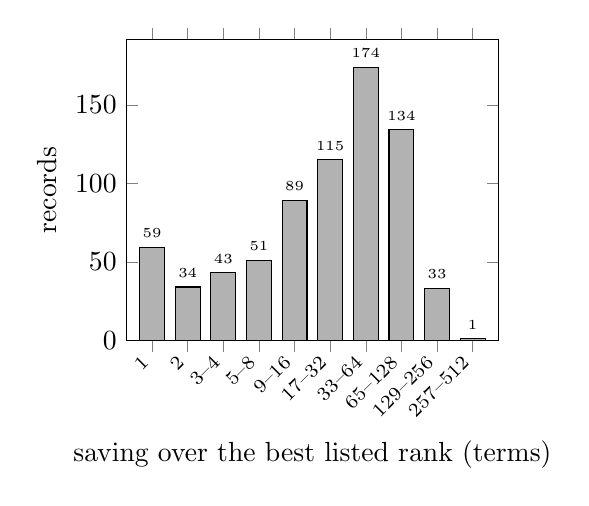
\begin{tikzpicture}
\begin{axis}[ybar,width=0.52\textwidth,height=5.4cm,bar width=9pt,ymin=0,
  symbolic x coords={1,2,3--4,5--8,9--16,17--32,33--64,65--128,129--256,257--512},xtick=data,
  xticklabel style={rotate=45,anchor=east,font=\scriptsize},xlabel={saving over the best listed rank (terms)},ylabel={records},
  nodes near coords,every node near coord/.append style={font=\tiny},enlarge x limits=0.08]
\addplot[fill=gray!60] coordinates {(1,59) (2,34) (3--4,43) (5--8,51) (9--16,89) (17--32,115) (33--64,174) (65--128,134) (129--256,33) (257--512,1)};
\end{axis}
\end{tikzpicture}\hfill
\begin{tikzpicture}
\begin{axis}[width=0.46\textwidth,height=5.4cm,xmode=log,xlabel={format volume $nmp$},ylabel={saving (\% of listed rank)},
  ymin=0,ymax=5.2,xmin=100,xmax=40000,legend style={at={(0.03,0.97)},anchor=north west,font=\scriptsize},mark size=1pt]
\addplot[only marks,mark=*,gray!75,mark options={fill=gray!60}] table[x=volume,y=relmargin] {data/scatter_nosearch.dat};
\addplot[only marks,mark=triangle*,black,mark size=1.4pt] table[x=volume,y=relmargin] {data/scatter_search.dat};
\legend{no walk or projection in the lineage,walk or projection}
\end{axis}
\end{tikzpicture}
\caption{Left: distribution of the saving over the best listed rank for the 733 records below every listed rank (octave bins). Right: relative saving against format volume for all 795 records, against the bar that defines each record's class.}
\label{fig:margins}
\end{figure}

\paragraph{The listed ranks for large formats are weak.}
92\% of the records have a side above 16, where the tables' entries are mostly not the result of a direct search but of composition over arbitrary rings (for 93.5\% of the 4{,}776 formats with a side above 16 the best rank the matmulcatalog lists is a derived entry, not an explicit scheme). A large saving against such an entry says that the entry is weak for $\F$, not that we found something hard.
The ordering of formats by saving shows it: the ten largest absolute savings (\cref{tab:top}) are all formats with a smallest side of 19 to 23 and a largest side of 27 to 32, nine of them July or committed certificates and one a projected closure product.
